%%%%%%%%%%%%%%%%%%%%%%%%%%%%%%%%%%%%%%%%%
% Masters/Doctoral Thesis 
% LaTeX Template
% Version 2.3 (25/3/16)
%
% This template has been downloaded from:
% http://www.LaTeXTemplates.com
%
% Version 2.x major modifications by:
% Vel (vel@latextemplates.com)
%
% This template is based on a template by:
% Steve Gunn (http://users.ecs.soton.ac.uk/srg/softwaretools/document/templates/)
% Sunil Patel (http://www.sunilpatel.co.uk/thesis-template/)
%
% Template license:
% CC BY-NC-SA 3.0 (http://creativecommons.org/licenses/by-nc-sa/3.0/)
%
%%%%%%%%%%%%%%%%%%%%%%%%%%%%%%%%%%%%%%%%%

%----------------------------------------------------------------------------------------
%	PACKAGES AND OTHER DOCUMENT CONFIGURATIONS
%----------------------------------------------------------------------------------------

\documentclass[
11pt, % The default document font size, options: 10pt, 11pt, 12pt
%oneside, % Two side (alternating margins) for binding by default, uncomment to switch to one side
%chapterinoneline,% Have the chapter title next to the number in one single line
%english, % ngerman for German
spanish,
singlespacing, % Single line spacing, alternatives: onehalfspacing or doublespacing
%draft, % Uncomment to enable draft mode (no pictures, no links, overfull hboxes indicated)
%nolistspacing, % If the document is onehalfspacing or doublespacing, uncomment this to set spacing in lists to single
%liststotoc, % Uncomment to add the list of figures/tables/etc to the table of contents
%toctotoc, % Uncomment to add the main table of contents to the table of contents
parskip, % Uncomment to add space between paragraphs
%nohyperref, % Uncomment to not load the hyperref package
headsepline, % Uncomment to get a line under the header
]{MastersDoctoralThesis} % The class file specifying the document structure



\usepackage[utf8]{inputenc} % Required for inputting international characters
\usepackage[T1]{fontenc} % Output font encoding for international characters

\usepackage{palatino} % Use the Palatino font by default
%,style=authoryear
\usepackage[backend=bibtex,natbib=true]{biblatex} % Use the bibtex backend with the authoryear citation style (which resembles APA)

\addbibresource{references.bib} % The filename of the bibliography

\usepackage[autostyle=true]{csquotes} % Required to generate language-dependent quotes in the bibliography

\usepackage{caption}
\usepackage{subcaption}

\usepackage{rotating}
\usepackage{tikz}

%------------------------
\usepackage{listings}

%\usepackage[hyphens]{url}
%\usepackage[hidelinks]{hyperref}
%\hypersetup{breaklinks=true}
\urlstyle{same}
%\usepackage{cite}

%--------------------------

\usepackage{color}

%
%----------------------------------------------------------------------------------------
%	MARGIN SETTINGS
%----------------------------------------------------------------------------------------

\geometry{
	paper=a4paper, % Change to letterpaper for US letter
	inner=2cm, % Inner margin
	outer=3.3cm, % Outer margin
	bindingoffset=2cm, % Binding offset
	top=1.5cm, % Top margin
	bottom=1.5cm, % Bottom margin
	%showframe,% show how the type block is set on the page
}

%----------------------------------------------------------------------------------------
%	INFORMACIÓN DE LA MEMORIA
%----------------------------------------------------------------------------------------

\thesistitle{Sistema de adquisición portátil de parámetros biomédicos para animales grandes} % El títulos de la memoria, se usa en la carátula y se puede usar el cualquier lugar del documento con el comando \ttitle
\supervisor{Dr. Ing. Damian Craiem Universidad Favaloro)} % El nombre del director, se usa en la carátula y se puede usar el cualquier lugar del documento con el comando \supname
\degree{Especialista en Sistemas Embebidos } % Nombre del grado, se usa en la carátula y se puede usar el cualquier lugar del documento con el comando \degreename
\author{Ing. Federico Roux} % Tu nombre, se usa en la carátula y se puede usar el cualquier lugar del documento con el comando \authorname
\juradoUNO{Dr. Ing. Mariano Casciaro (CONICET - Fundación Favaloro)} % Nombre y pertenencia del un jurado se usa en la carátula y se puede usar el cualquier lugar del documento con el comando \jur1name
\juradoDOS{Esp. Ing. Jerónimo La Bruna (FIUBA)} % Nombre y pertenencia del un jurado se usa en la carátula y se puede usar el cualquier lugar del documento con el comando \jur2name
\juradoTRES{Ing. Manuel Alfonso (UTN.BA)} % Nombre y pertenencia del un jurado se usa en la carátula y se puede usar el cualquier lugar del documento con el comando \jur3name
\fechaINICIO{mayo de 2018}
\fechaFINAL{diciembre de 2018}

\subject{Memoria del Trabajo Final de la Carrera de Especialización en Sistemas Embebidos de la UBA} % Your subject area, this is not currently used anywhere in the template, print it elsewhere with \subjectname
\keywords{CESE, Sistemas Embebidos, CIAA} % Keywords for your thesis, this is not currently used anywhere in the template, print it elsewhere with \keywordnames
\university{Universidad de Buenos Aires} % Your university's name and URL, this is used in the title page and abstract, print it elsewhere with \univname
\faculty{{Facultad de Ingeniería}} % Your faculty's name and URL, this is used in the title page and abstract, print it elsewhere with \facname
\department{Departamento de Electrónica} % Your department's name and URL, this is used in the title page and abstract, print it elsewhere with \deptname
\group{{Laboratorio de Sistemas Embebidos}} % Your research group's name and URL, this is used in the title page, print it elsewhere with \groupname


\hypersetup{pdftitle=\ttitle} % Set the PDF's title to your title
\hypersetup{pdfauthor=\authorname} % Set the PDF's author to your name
\hypersetup{pdfkeywords=\keywordnames} % Set the PDF's keywords to your keywords


\newcaptionname{spanish}{\acknowledgementname}{Agradecimientos}
\newcaptionname{spanish}{\authorshipname}{Declaración de Autoría}
\newcaptionname{spanish}{\abbrevname}{Glosario}
\newcaptionname{spanish}{\byname}{por}

\renewcommand{\lstlistingname}{Algoritmo}% Listing -> Algorithm
\renewcommand{\lstlistlistingname}{Índice de \lstlistingname s}% List of Listings -> List of Algorithms

\renewcommand{\listtablename}{Índice de Tablas}
\renewcommand{\tablename}{Tabla} 

\addtolength{\footnotesep}{2mm} % Espacio adicional en los footnotes

\begin{document}

\frontmatter % Use roman page numbering style (i, ii, iii, iv...) for the pre-content pages

\pagestyle{plain} % Default to the plain heading style until the thesis style is called for the body content

%----------------------------------------------------------------------------------------
%	CARÁTULA
%----------------------------------------------------------------------------------------

\begin{titlepage}
\begin{center}

{\scshape\LARGE UNIVERSIDAD DE BUENOS AIRES\par}\vspace{0.1cm} % University name
{\scshape\LARGE FACULTAD DE INGENIERÍA\par}\vspace{0.1cm} % Faculty name
{\scshape\LARGE Carrera de Especialización en Sistemas Embebidos\par}\vspace{1cm} % Thesis type


\includegraphics[width=.3\textwidth]{./Figures/logoFIUBA.png}
\vspace{1cm}

\textsc{\Large Memoria del Trabajo Final}\\[0.5cm] % Thesis type

{\huge \bfseries \ttitle\par}\vspace{0.4cm} % Thesis title

\vspace{1cm}
\LARGE\textbf{Autor:\\
\authorname}\\ % Author name

\vspace{1cm}

\large
\vspace{10px}
{Director:} \\
{\supname} % Supervisor name
 
\vspace{1cm}
Jurados:\\
\jurunoname\\
\jurdosname\\
\jurtresname
 
\vfill
\textit{Este trabajo fue realizado en las Ciudad Autónoma de Buenos Aires, entre \fechaINICIOname \hspace{1px} y \fechaFINALname.}
\end{center}
\end{titlepage}


%----------------------------------------------------------------------------------------
%	RESUMEN - ABSTRACT 
%----------------------------------------------------------------------------------------

\begin{abstract}
\addchaptertocentry{\abstractname} % Add the abstract to the table of contents
%
%The Thesis Abstract is written here (and usually kept to just this page). The page is kept centered vertically so can expand into the blank space above the title too\ldots
\centering

En la presente memoria se describe el desarrollo de un sistema de adquisición portátil para medición de parámetros biomédicos en animales grandes. En particular, se tiene interés en la medición de la velocidad de onda de pulso (VOP), cuyo método más aceptado de cálculo consiste en el registro simultáneo de señales de presión intraarterial en dos puntos del árbol arterial. Conociendo la distancia y el desfasaje temporal entre estas mediciones de presión, se puede estimar la VOP como su cociente.

Para este proyecto se utilizaron en forma intensiva la gran mayoría de los contenidos y herramientas vistas durante el Curso de Especialización CESE. Se utilizaron técnicas de Gestión de Proyectos, documentación manual y automática del trabajo, sistema de versionado de software y hardware. En cuanto a lo técnico se emplearon conocimientos específicos sobre arquitectura del microcontrolador, modelos de programación, sistema operativo de tiempo real freeRTOS, protocolos de comunicación (BLE, SPI, USB, y de alto nivel), testing unitarios, etc.

\end{abstract}

%----------------------------------------------------------------------------------------
%	CONTENIDO DE LA MEMORIA  - AGRADECIMIENTOS
%----------------------------------------------------------------------------------------

\begin{acknowledgements}
%\addchaptertocentry{\acknowledgementname} % Descomentando esta línea se puede agregar los agradecimientos al índice
\vspace{1.5cm}

%Agradecimientos personales. 

Se agradece especialmente al director de este proyecto, Dr. Ing. Damián Craiem y a su equipo de trabajo, por el esfuerzo y dedicación diarias en la investigación, los cuales generan nuevos campos de aplicación de la ingeniería electrónica. Y en particular por la continuidad de este proyecto a través del tiempo y la oportunidad de poder participar en el mismo.

\end{acknowledgements}

%----------------------------------------------------------------------------------------
%	LISTA DE CONTENIDOS/FIGURAS/TABLAS
%----------------------------------------------------------------------------------------
\renewcommand{\listtablename}{Índice de Tablas}

\tableofcontents % Prints the main table of contents

\listoffigures % Prints the list of figures

\listoftables % Prints the list of tables


%----------------------------------------------------------------------------------------
%	CONTENIDO DE LA MEMORIA  - DEDICATORIA
%----------------------------------------------------------------------------------------

% \dedicatory{\textbf{Dedicado a... [OPCIONAL]}}  % escribir acá si se desea una dedicatoria

%----------------------------------------------------------------------------------------
%	CONTENIDO DE LA MEMORIA  - CAPÍTULOS
%----------------------------------------------------------------------------------------

\mainmatter % Begin numeric (1,2,3...) page numbering

\pagestyle{thesis} % Return the page headers back to the "thesis" style

\renewcommand{\tablename}{Tabla} 

% Incluir los capítulos como archivos separados desde la carpeta Chapters
% Descomentar las líneas a medida que se escriben los capítulos

% Chapter 1

\chapter{Introducción General} % Main chapter title

\label{Chapter1} % For referencing the chapter elsewhere, use \ref{Chapter1} 
\label{IntroGeneral}

%----------------------------------------------------------------------------------------

% Define some commands to keep the formatting separated from the content 
\newcommand{\keyword}[1]{\textbf{#1}}
\newcommand{\tabhead}[1]{\textbf{#1}}
\newcommand{\code}[1]{\texttt{#1}}
\newcommand{\file}[1]{\texttt{\bfseries#1}}
\newcommand{\option}[1]{\texttt{\itshape#1}}
\newcommand{\grados}{$^{\circ}$}

%----------------------------------------------------------------------------------------

\section{Introducción}

En el presente capítulo se describen los lineamientos generales del trabajo, sus motivaciones en el campo de la Ingeniería Biomédica, el estado del arte actual y los objetivos específicos alcanzados.


%----------------------------------------------------------------------------------------
\section{Descripcion General del Trabajo}

El trabajo aquí presentado consiste en un sistema de adquisición portátil para medición de parámetros biomédicos en animales grandes. Se tiene particular interés en la medición del parámetro biológico denominado \enquote{velocidad de onda de pulso (VOP)}, cuyo método de cálculo más aceptado consiste en el registro simultáneo de señales de presión intraarterial en dos puntos del árbol arterial. Conociendo la distancia y el desfasaje temporal entre estas mediciones de presión, se puede estimar la VOP como su cociente. Esto puede verse graficado en la figura \ref{fig:vop}.

\begin{figure}[!htbp]
	\centering
	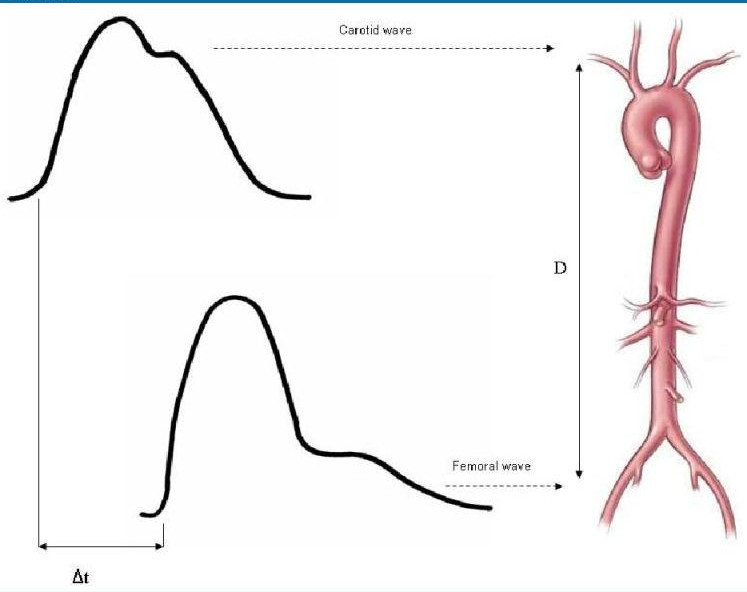
\includegraphics[width=\textwidth]{./Figures/VOP.jpg}
	\caption{Medición de VOP a partir de dos mediciones de la curva de presión, con un desfasaje temporal conocido}
	\label{fig:vop}
\end{figure}

El dispositivo desarrollado en este trabajo está orientado a ser utilizado por investigadores médicos, ingenieros biomédicos, biólogos y veterinarios en grupos de trabajo en general aplicado a cardiología. En particular este trabajo se realiza para la Universidad Favaloro, y es importante porque permitirá avanzar a futuro en el conocimiento de formas de medición de presión ambulatoria indirecta, más precisas y menos invasivas.

\subsection{Bases físicas de la medición}

De acuerdo a la Organización Mundial de la Salud, la presión sanguínea humana es medida de la presión que ejerce la sangre circulante sobre las paredes de los vasos sanguíneos \cite{who2015}. Esta onda de presión es originada por el latido del corazón y transmitida hacia todo el árbol arterial. La composición entre la onda incidente y la reflejada dan origen a la onda estacionaria de presión, cuyo máximo y mínimo dan origen a los valores característicos conocidos como \textbf{presion sistólica} y \textbf{presión diastólica}. Estos valores tienen una gran importancia en la clínica. En un adulto sano, estos valores son aproximadamente 120mmHg para la presión sistólica y 80mmHg para la presión diastólica. En la figura \ref{fig:periodopresion} puede observarse una forma de onda característica.

\begin{figure}[!htbp]
	\centering
	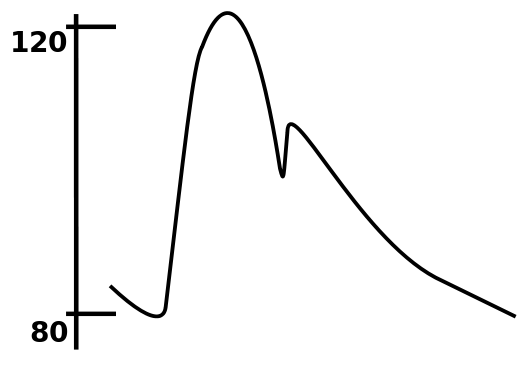
\includegraphics[width=\textwidth]{./Figures/periodopresion.png}
	\caption{Forma de onda de un ciclo de una señal de presión humana típica}
	\label{fig:periodopresion}
\end{figure}


\subsection{Estado del arte}

La medición ambulatoria de presión arterial (MAPA) braquial durante 24 horas es un método ampliamente aceptado para predecir riesgo cardiovascular y mortalidad\citep{hansen2006} \citep{staensen1999} \citep{verdecchia1993}. Se sabe que la variabilidad de la presión arterial y su pulsatilidad son el resultado de una compleja interacción entre el corazón y la red vascular. En particular, y para la evaluación de las características biomecánicas de la red arterial, se utiliza la velocidad de onda de pulso (VOP) como indicador indirecto de rigidez arterial \citep{nichols2008}.

Actualmente, existen diferentes técnicas para la medición de presión \citep{ogedegbe2010}. Pueden agruparse entre los métodos que brindan mediciones puntuales (presión sistólica, diastólica y media) y los que brindan mediciones contínuas. Entre los que brindan mediciones puntuales están el método auscultatorio, el método oscilométrico, método palpatorio, técnicas de ultrasonido, etc. Por otro lado, los que brindan mediciones contínuas suelen ser métodos invasivos como el catéter o no invasivos como la medición indirecta a partir de la medición de VOP \citep{ruso2001}.

La técnica más utilizada y difundida en la medicina clínica es el método oscilométrico, que basa su funcionamiento en monitorear las variaciones de la señal de presión en una banda inflable que se aplica alrededor del brazo izquierdo, logrando determinal a través del análisis de esta señal los valores de presión sistólica, diastólica y media de los pacientes. Mientras la banda se desinfla desde un nivel por encima de la presión sistólica, las paredes de la arteria comienzan a oscilar a medida que la sangre fluye a través del vaso parcialmente ocluído, y estas vibraciones son captadas en el transductor que monitorea la presión en la banda. Cuando la presión en la banda sigue disminuyendo, las oscilaciones aumentan hasta una amplitud máxima y luego disminuyen  hasta que la banda se desinfla completamente y el flujo de sangre regresa a la normalidad.

La presión en la banda en el punto de máxima oscilación normalmente se corresponde con la presión arterial media \ref{fig:moscilometrico}. El punto por encima de la presión media, en el cual las oscilaciones comienzan rápidamente a aumentar en amplitud se corresponde con la presión sistólica. El punto en que esta variación de las oscilaciones disminuye de forma más abrupta, se corresponde con la presión diastólica. Este método es de gran utilidad para la medicina clínica hace muchos años, sin embargo, tiene la contrapartida de que se pierde el detalle de la forma de onda de la curva de presión, lo cual es solo posible apreciar utilizando un sistema de adquisición contínuo con una tasa de muestreo adecuada.


\begin{figure}[!htbp]
	\centering
	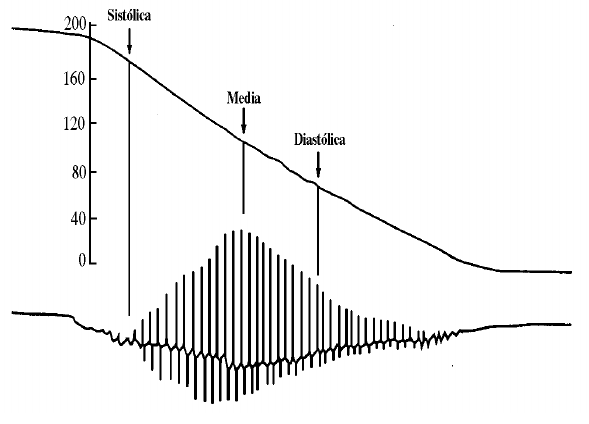
\includegraphics[width=\textwidth]{./Figures/moscilometrico.png}
	\caption{Curva de inflado de la almohadilla de método del MAPA más utilizado vs presión real.\\ Presión diferencial medida y ruidos detectados.}
	\label{fig:moscilometrico}
\end{figure}

Es claro que la medición de la onda contínua aporta muchos más datos que la medición de puntos característicos de la curva. A partir de la onda completa, se pueden calcular diferentes parámetros que permiten modelizar el árbol arterial y predecir enfermedades como hipertensión, arteriosclerosis, rigidez arterial, etc \citep{saito2011}  \citep{figueroa2014}.


\subsection{Medicion ambulatoria de presión arterial}

Una de las técnicas para medición contínua de presión es la medición indirecta a partir del VOP. El método más aceptado para medir VOP en pacientes consiste en el registro simultáneo de señales de presión en carótida y femoral. Conociendo la distancia y el desfasaje temporal entre estas mediciones de presión, se puede estimar la VOP como su cociente. La medición de VOP ha ingresado en las últimas guías de recomendación europeas como indicadora (Clase IIa; Nivel de evidencia B) para la evaluación subclínica de daño en órganos en pacientes hipertensos. El interés clínico en esta medición ha llevado al desarrollo de numerosos dispositivos para medir VOP y cuyas características y limitaciones están siendo analizadas actualmente para hallar un estándar internacional \citep{laurent2006} Así como la MAPA braquial ha impulsado el desarrollo de dispositivos de registro y análisis cada vez más sofisticados, la posibilidad de realizar un registro ambulatorio de VOP genera nuevos campos de investigación, así como la necesidad de que existan nuevos dispositivos \citep{omboni2016}.


Existen otros metodos de estimacion de la MAPA, pero se generan numerosas controversias debido a la complejidad matemática de las estimaciones y al uso de modelos matemáticos  arteriales unificados que suponen ser válidos para todos los pacientes. 
La presión arterial humana responde a una curva que tiene un pico y un valle, y una forma de onda característica. De esta curva pueden calcularse toda una serie de parámetros que modelizan el arbol arterial. Sin embargo, el método más utilizado en la medicina clínica para estimar la presión arterial, el método oscilométrico, solo toma dos valores característicos de esta curva, el máximo y el mínimo, denominados presion sistólica y presión diastólica.

\section{Motivación y Aplicaciones del equipo}

En este contexto, el estudio ambulatorio de la VOP en animales grandes podría brindar nuevas oportunidades para validar diferentes algoritmos de cálculo. La adquisición invasiva de señales de presión en dos sitios alejados del sistema arterial y a una distancia conocida, permite mejorar el conocimiento actual sobre la VOP en distintas condiciones del animal.

Las experiencias realizadas con este equipo permitirán profundizar la investigación sobre la medición indirecta de presión ambulatoria a partir de la medición de VOP y las técnicas para su cálculo. La aplicación de esta técnica para la MAPA permitirá desarrollar a futuro equipos portátiles que puedan medir de manera continua la presión de un paciente, con más información, mejor resolución y más comodidad.

Las experiencias de medición de VOP se realizan sobre animales grandes concientes, como ovejas o cerdos. Estos animales se encuentran previamente instrumentados con sensores de presión intraarteriales en forma crónica y tienen un prolongado período de adaptación a la vida en un corral de un laboratorio de investigación y al trato con los veterinarios. En la figura \ref{fig:oveja} puede verse una fotografía de una oveja durante una experiencia real con un equipamiento antiguo. La correcta adaptación del animal a la vida en el corral del laboratorio es muy importante porque la presión arterial se ve severamente afectada por la comodidad y bienestar del animal. Por ejemplo, algunas de las líneas de investigación estudian justamente la diferencia de los valores medios de presión entre el período de vigilia y de sueño. Este tipo de experiencias sobre un animal en estado de alerta se hace totalmente imposible.


\begin{figure}[!htbp]
	\centering
	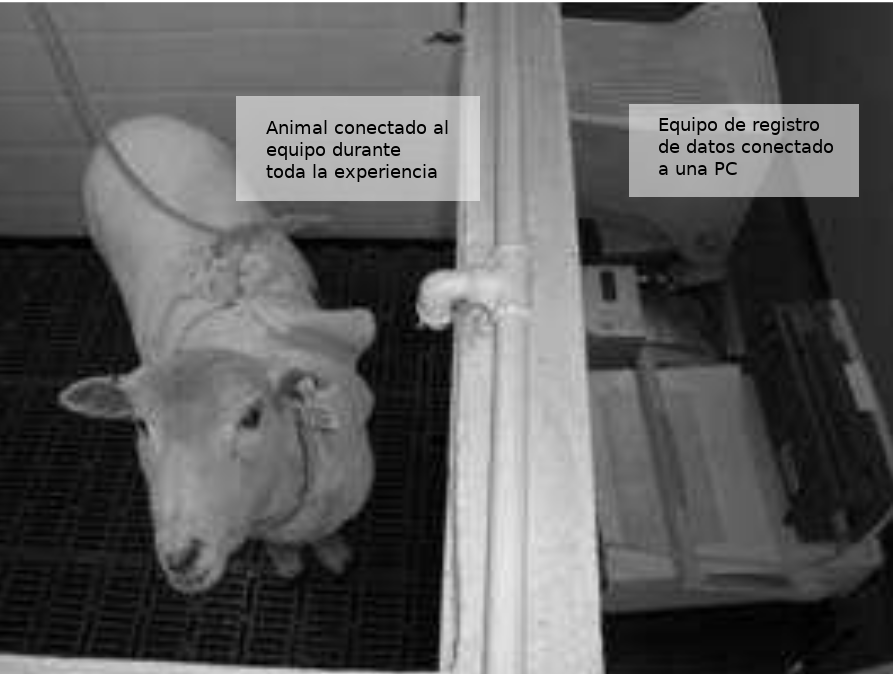
\includegraphics[width=\textwidth]{./Figures/oveja.png}
	\caption{Oveja instrumentada con un equipamiento antiguo con interfaz cableada. En la derecha de la imagen se puede observar el equipo de registro de datos antiguo, el cual depende de una PC y obliga a tener el animal conectado al equipo mediante un cable durante toda la experiencia.}
	\label{fig:oveja}
\end{figure}

El equipamiento de medición debe ir sobre el animal para evitar que existan cables que limiten el movimiento y dificulten la vida diaria del mismo. Además, luego de un período de adaptación, el equipo debe ser imperceptible para el animal. Esto se logra con un tamaño reducido, un sistema de carga cómoda, como una pequeña mochila, bajo peso, ausencia de ruido, etc. Durante toda la experiencia de medición, el equipo debe estar sobre el animal, y, en lo posible, solo debe acercarse personal de veterinaria para tareas de higiene y alimentación. El operador del equipo debería solamente acercarse al animal para la instalación del equipo, y para retirarlo al finalizar la experiencia. El resto del tiempo, el operador debe tener una interacción mínima con el animal.


\section{Objetivos y alcance}

El proyecto incluyó el desarrollo completo de un dispositivo de medición y adquisición de dos sensores de presión intraarteriales para ser utilizado en animales grandes, junto con su documentación técnica y manual de usuario. 

Las señales además se pueden visualizar en tiempo real para realizar algún eventual ajuste sobre el animal instrumentado antes de comenzar la experiencia. Este software de visualización no se incluye entre los alcances del proyecto, por lo que se utiliza solamente una interfaz en desarrollo a modo de prueba. 

El equipo se diseñó para ser portátil, alimentado por batería, con una autonomía aproximada de 24 horas. A la vez, se hizo énfasis en lograr un bajo peso que no moleste al animal durante la experiencia. La interfaz de carga es a través de la misma conexión USB.

El desarrollo del proyecto no incluye la fabricación del gabinete final ni del soporte para ser llevado por el animal. Tampoco se incluye el software de la terminal de configuración, solamente una versión preliminar para pruebas.

%----------------------------------------------------------------------------------------

\chapter{Introducción Específica} % Main chapter title

\label{Chapter2}

%----------------------------------------------------------------------------------------
%	SECTION 1
%----------------------------------------------------------------------------------------
Este proyecto se destaca principalmente por ser un sistema de adquisición diseñado especialmente para realizar experiencias en animales grandes sin alterar su comportamiento durante lapsos prolongados, para evitar incidir sobre los valores de tensión arterial medidos. Para ello, se invirtió esfuerzo en lograr un equipo de pequeño tamaño y bajo peso, y a la vez se trabajó en la necesidad de contar con una interfaz de usuario inalámbrica que me permita configurar el equipo y chequear esporádicamente su funcionamiento evitando que el operador se acerque al animal. 

El equipo diseñado digitaliza las señales analógicas y las guarda en una memoria flash de almacenamiento masivo (SD) durante períodos de tiempo prolongados, de aproximadamente 24hs. Puede configurarse y controlarse desde una terminal remota a través de una interfaz comunicada por BLE.

\section{Detalle de las necesidades}

Las experiencias de medición consisten básicamente en colocar el equipo en una especie de pequeña mochila que se ajusta sobre el animal instrumentado. Una vez que está instalado, el equipo adquiere durante un período de alrdededor de 24hs. Esto da un margen de tiempo para que el animal se tranquilice luego de la instalación del dispositivo, normalice su comportamiento, y pase por diferentes fases a lo largo del día: vigilia, sueño, alimentación, interacción con veterinarios, etc. 

La presión arterial es un parámetro que es fuertemente dependiente del bienestar del animal, por lo que es importante que la batería tenga autonomía suficiente para toda la experiencia y que no sea necesario intercambiar ni recambiar las baterías. De esto también peude deducirse que el equipo debe ser portátil para que el animal no esté conectado a ningún equipo a través de cables. Como se trata de una experiencia larga, también es importante que el equipo no sea pesado, voluminoso, ruidoso, ni se caliente. 

Los sensores utilizados son del tipo strain-gauge. Pueden visualizarse en la imagen \ref{fig:konigsberg}. Se trata de una resistencia que varía su valor de acuerdo a la presión aplicada. El sensor además cuenta con propiedades aptas para ser implantado en un animal. Este sensor tiene un conector propio de la marca Konigsberg al que se le conecta un compensador por temperatura calibrado específicamente para cada sensor, y de allí se utiliza un conector estándar roscado Amphenol de 4 pines dorados para ingresar al equipo. Esta última conexión es muy importante para evitar que se agregue ruido a la señal medida.

\begin{figure}[!htbp]
	\centering
	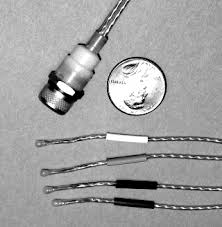
\includegraphics[width=\textwidth]{./Figures/konigsberg.jpeg}
	\caption{Imagen de conector, cable y sensor konigsberg}
	\label{fig:konigsberg}
\end{figure}

La señal de presión arterial tiene un patrón normal con diferentes puntos característicos. Puede observarse en la figura \ref{fig:senpresion} un gráfico típico de una señal de presión arterial de un mamífero. La forma de la curva corresponde a una onda estacionaria conformada por una señal incidente pulsátil y una onda reflejada, y puede analizarse como un sistema de parámetros distribuídos. Tiene una frecuencia fundamental apenas superior a 1Hz, sin embargo, contiene componentes de frecuencia hasta los 100Hz, con los que es necesario contar para obtener una buena resolucón en el momento de realizar el análisis de la forma de onda. Una frecuencia de muestreo típica utilizada para adquirir este tipo de señales es \textbf{500Hz} o \textbf{1kHz}. Una excursión normal de una señal de presión de un ser humano puede tener un máximo de 140mmHg, por lo que es útil contar con un rango dinámico mayor a este, por ejemplo 200mmHg. Una adquisición con una resolución del 0.5\%, es decir, de 1mmHg sería adecuada.

\begin{figure}[!htbp]
	\centering
	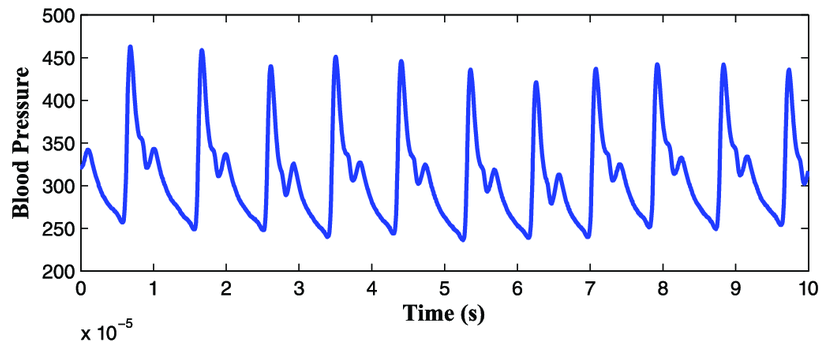
\includegraphics[width=\textwidth]{./Figures/senpresion.png}
	\caption{Señal típica de presión arterial de un mamífero.}
	\label{fig:senpresion}
\end{figure}

Es muy común que antes de comenzar la experiencia, o durante la experiencia, el animal se mueva o intente tocar los cables que van desde los sensores hasta la mochila donde se encuentra alojada el equipo. Estos movimientos pueden ocasionar cambios en el estado de las conexiones de los sensores, o eventualmente, en el estado del equipo. Es útil, desde el punto de vista del operador del equipo, poder tener algún tipo de información sobre la señal que se está midiendo, de manera de saber si es necesario realizar algún ajuste en las conexiones. Sin embargo, esta observación debe ser idealmente sin molestar al animal, es decir en forma inalámbrica. También puede suceder que los sensores puedan moverse, y por lo tanto, sufran algún tipo de cambio en su ganancia, que deba ser ajustada desde el circuito analógico para no perder resolución. 
Finalmente, una vez comenzada la medición, al tratarse de una experiencia tan costosa en cuanto a recursos y tiempo, es importante poder controlar esporádicamente que la adquisición se esté realizando de forma correcta, sin afectar el comportamiento del animal. Por lo tanto es muy útil desde el punto de vista operativo de recursos poder visualizar la señal que se está adquiriendo en forma remota sin influir en el animal, es decir, de forma remota.


\section{Requerimientos}

En base a todo lo comentado en la sección anterior, se desprenden los siguientes requerimientos asociados de acuerdo a criterios de energía, tamaño y peso, conectividad y adquisición, con los que fue desarrollado el equipo:


\begin{enumerate}
	\item \textbf{Necesidades asociadas a la alimentación:} 
	\begin{enumerate}
		\item El equipo debe tener una autonomía mayor a 24 horas en el modo de adquisición y almacenamiento, a una dada frecuencia de muestreo.
		\item El equipo debe ser portátil e inalámbrico, por lo tanto, alimentado a batería
	\end{enumerate}
	
	\item \textbf{Requerimientos asociados al tamaño físico del equipo:}
	\begin{enumerate}
		\item El peso del equipo debe tener un peso aproximado de 500 gr
		\item El tamaño debe ser aproximadamente de 10cm x 10cm
		\item El equipo no debe calentarse demasiado
	\end{enumerate}
	
	\item \textbf{Requerimientos asociados a la conectividad e interfaz de usuario:}
	
	\begin{enumerate}
		\item Se deben poder visualizar las señales medidas en tiempo real previo a iniciar la experiencia.
		\item Se debe realizar la configuración de la adquisición (ganancia, canales habilitados, frecuencia de muestreo, etc.) desde una terminal Bluetooth.
		\item Se debe poder acceder a la memoria SD a través de la conexión USB.
	\end{enumerate}


	\item \textbf{Requerimientos asociados a la adquisición y almacenamiento:}
	
	\begin{enumerate}
		\item El equipo debe tener una resolución de 1 mmHg en alguna de las escalas de ganancia.
		\item Debe poder manejar almacenamiento suficiente para la máxima resolución elegida y frecuencia de muestreo.
		\item Se debe poder configurar el tamaño de muestra.
	\end{enumerate}

\end{enumerate}


\section{Planificación}

En las siguientes figuras, \ref{fig:gantt1} y \ref{fig:gantt2}, puede observarse la planificación original del trabajo en un diagrama de Gantt. 

\begin{figure}[!htbp]
	\centering
	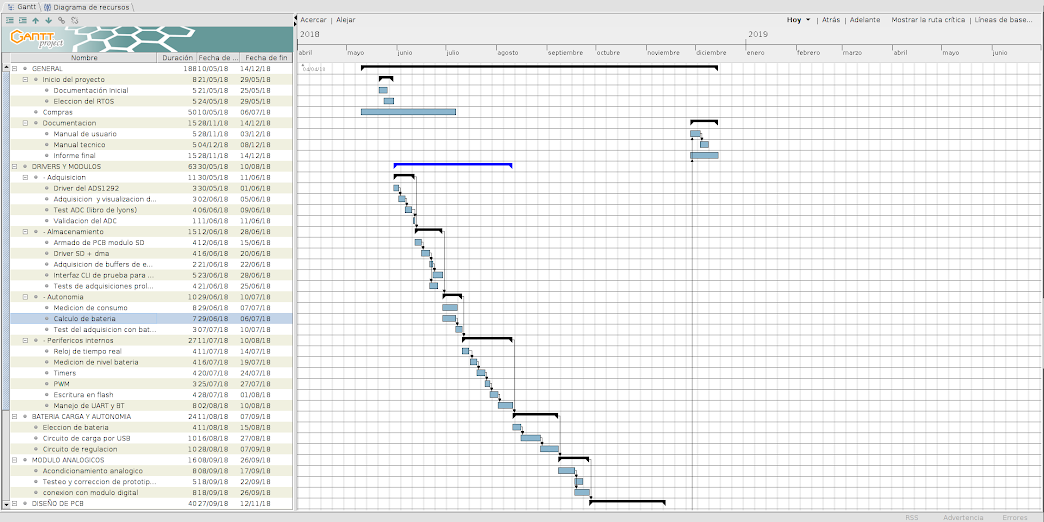
\includegraphics[width=\textwidth]{./Figures/gantt1.png}
	\caption{Diagrama de gantt - Primer parte}
	\label{fig:gantt1}
\end{figure}

\begin{figure}[!htbp]
	\centering
	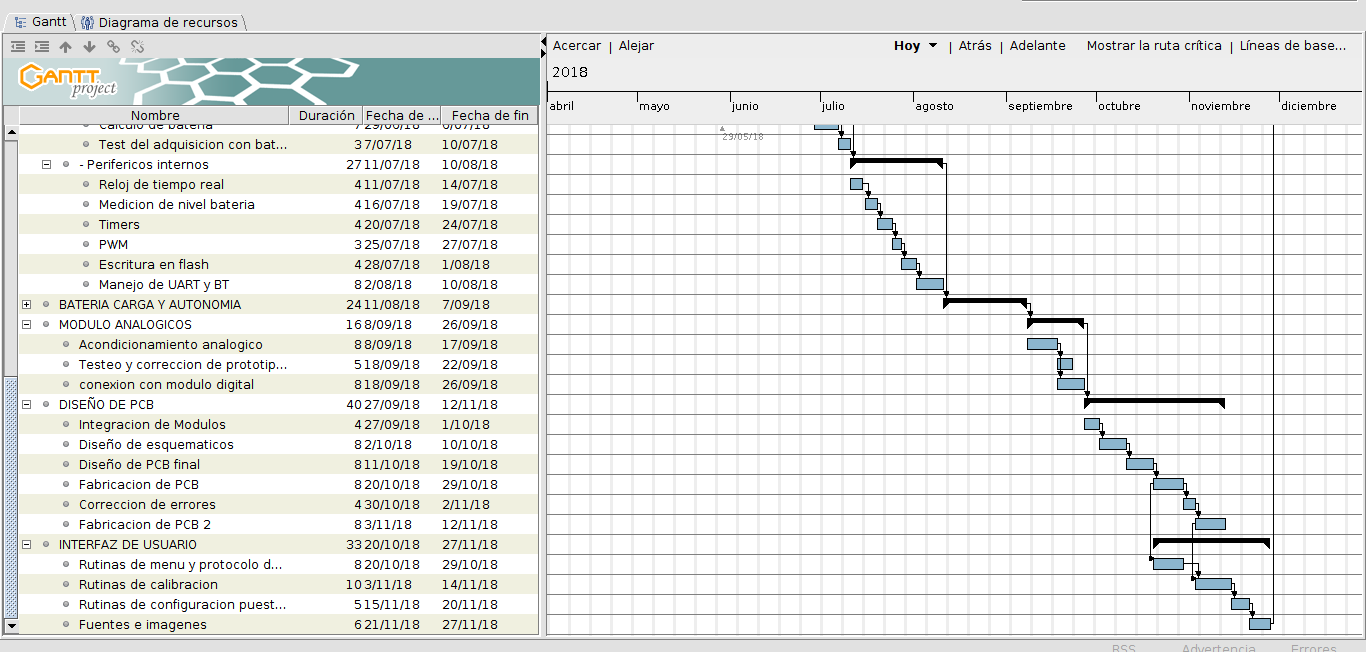
\includegraphics[width=\textwidth]{./Figures/gantt2.png}
	\caption{Diagrama de gantt - Segunda parte}
	\label{fig:gantt2}
\end{figure}

En este diagrama puede verse una organización del trabajo en los siguientes módulos de trabajo:

\begin{enumerate}

\item \textbf{General:} Documentación inicial del proyecto, selección de rtos y microcontrolador, documentación de memoria técnica, manuales de usuario y técnico, presentaciones, compras de componentes, pedido de servicios, etc.

\item \textbf{Drivers y módulos:} driver del ADC, tests de adquisición, driver de almacenamiento, manejo del DMA, interfaz de prueba para configuración, programación de drivers de periféricos, etc.

\item \textbf{Batería, carga y autonomía:} medición de consumo, elección de batería, circuito de carga USB, circuito de regulación.

\item \textbf{Módulos analógicos:} acondicionamiento analógico de la señal, interconexión con módulo digital.

\item \textbf{Diseño de PCB:} integración de módulos, esquemáticos, diseño de PCB, fabricación, soldadura, etc.

\item \textbf{Interfaz de Usuario:} Rutinas de menú, protocolo de comunicación, configuración, fuentes, imágenes, testing unitarios, testing de sistema, etc.

\end{enumerate} 
\chapter{Diseño e Implementación} % Main chapter title

\label{Chapter3} % Change X to a consecutive number; for referencing this chapter elsewhere, use \ref{ChapterX}
\definecolor{mygreen}{rgb}{0,0.6,0}
\definecolor{mygray}{rgb}{0.5,0.5,0.5}
\definecolor{mymauve}{rgb}{0.58,0,0.82}

\lstset{ %
  backgroundcolor=\color{white},   % choose the background color; you must add \usepackage{color} or \usepackage{xcolor}
  basicstyle=\footnotesize,        % the size of the fonts that are used for the code
  breakatwhitespace=false,         % sets if automatic breaks should only happen at whitespace
  breaklines=true,                 % sets automatic line breaking
  captionpos=b,                    % sets the caption-position to bottom
  commentstyle=\color{mygreen},    % comment style
  deletekeywords={...},            % if you want to delete keywords from the given language
  %escapeinside={\%*}{*)},          % if you want to add LaTeX within your code
  %extendedchars=true,              % lets you use non-ASCII characters; for 8-bits encodings only, does not work with UTF-8
  %frame=single,	                   % adds a frame around the code
  keepspaces=true,                 % keeps spaces in text, useful for keeping indentation of code (possibly needs columns=flexible)
  keywordstyle=\color{blue},       % keyword style
  language=[ANSI]C,					% the language of the code
  %otherkeywords={*,...},           % if you want to add more keywords to the set
  numbers=left,                    % where to put the line-numbers; possible values are (none, left, right)
  numbersep=5pt,                   % how far the line-numbers are from the code
  numberstyle=\tiny\color{mygray}, % the style that is used for the line-numbers
  rulecolor=\color{black},         % if not set, the frame-color may be changed on line-breaks within not-black text (e.g. comments (green here))
  showspaces=false,                % show spaces everywhere adding particular underscores; it overrides 'showstringspaces'
  showstringspaces=false,          % underline spaces within strings only
  showtabs=false,                  % show tabs within strings adding particular underscores
  stepnumber=1,                    % the step between two line-numbers. If it's 1, each line will be numbered
  stringstyle=\color{mymauve},     % string literal style
  tabsize=2,	                   % sets default tabsize to 2 spaces
  title=\lstname,                   % show the filename of files included with \lstinputlisting; also try caption instead of title
  morecomment=[s]{/*}{*/}%
}


%----------------------------------------------------------------------------------------
%	SECTION 1
%----------------------------------------------------------------------------------------
\section{Análisis del software}
 
La idea de esta sección es resaltar los problemas encontrados, los criterios utilizados y la justificación de las decisiones que se hayan tomado.

Se puede agregar código o pseudocódigo dentro de un entorno lstlisting con el siguiente código:

\begin{verbatim}
\begin{lstlisting}[caption= "un epígrafe descriptivo"]

	las líneas de código irían aquí...
	
\end{lstlisting}
\end{verbatim}

A modo de ejemplo:

\begin{lstlisting}[caption=Pseudocódigo del lazo principal de control.]  % Start your code-block

#define MAX_SENSOR_NUMBER 3
#define MAX_ALARM_NUMBER  6
#define MAX_ACTUATOR_NUMBER 6

uint32_t sensorValue[MAX_SENSOR_NUMBER];		
FunctionalState alarmControl[MAX_ALARM_NUMBER];	//ENABLE or DISABLE
state_t alarmState[MAX_ALARM_NUMBER];						//ON or OFF
state_t actuatorState[MAX_ACTUATOR_NUMBER];			//ON or OFF

void vControl() {

	initGlobalVariables();
	
	period = 500 ms;
		
	while(1) {

		ticks = xTaskGetTickCount();
		
		updateSensors();
		
		updateAlarms();
		
		controlActuators();
		
		vTaskDelayUntil(&ticks, period);
	}
}
\end{lstlisting}




% Chapter Template

\chapter{Ensayos y Resultados} % Main chapter title

\label{Chapter4} % Change X to a consecutive number; for referencing this chapter elsewhere, use \ref{ChapterX}

Este capítulo expone las características del dispositivo desarrollado en contraste con los requerimientos de diseño y los casos de uso.
%----------------------------------------------------------------------------------------
%	SECTION 1
%----------------------------------------------------------------------------------------

\section{Análisis de casos de uso y cumplimiento de los requerimientos}
\label{sec:pruebasHW}

\textbf{Caso de uso CU001: Autonomía}

El primer caso de uso analizado está relacionado a la autonomía del equipo. Se midió el consumo del equipo en diferentes situaciones en la que no está conectado por USB. Los resultados se muestran en la Tabla \ref{tab:autonomia}.

\begin{table}[h]
\caption{Autonomía del Equipo}
\label{tab:autonomia}
\begin{tabular}{@{}llll@{}}
\toprule
\textbf{Fase}                       & \textbf{\begin{tabular}[c]{@{}l@{}}Consumo\\ promedio\end{tabular}} & \textbf{\begin{tabular}[c]{@{}l@{}}Duración \\ estimada\end{tabular}} & \textbf{Descripción}                                                                                                \\ \midrule
En espera de conexión BT                  & I$_0$ = 78mA                                                         & t$_0$ = 30 min                                                         & \begin{tabular}[c]{@{}l@{}}Instalo el equipo y \\ conecto sensores\end{tabular}                                     \\
Configuración previa a experiencia  & I$_1$ = 65mA                                                         & t$_1$ = 30 min                                                          & \begin{tabular}[c]{@{}l@{}}Envío señal de prueba, \\ configuro parámetros\end{tabular}                              \\
Equipo conectado BT inactivo        & I$_2$ = 62 mA                                                        & t$_2$ = 10 min                                                          & \begin{tabular}[c]{@{}l@{}}Modificación de la \\ instalación del equipo \\ (sujeción, conectores, etc)\end{tabular} \\
Equipo adquiriendo sin enviar señal & I$_3$ = 45 mA                                                        & t$_3$ = 24 hs                                                           & Experiencia                                                                                                         \\
Acceso a ver señal                  & I$_4$ = 75 mA                                                       & t$_4$ = 20 min                                                           & \begin{tabular}[c]{@{}l@{}}Accedo eventualmente a \\ ver la señal que se está\\ adquiriendo\end{tabular}            \\ \bottomrule
\end{tabular}
\end{table}

Se calculó el consumo medio teórico realizando el promedio ponderado de los consumos en las situaciones presentadas en la Tabla \ref{tab:autonomia}. El resultado se presenta en la ecuación \ref{eqn:consumoMedio}.

\begin{equation} \label{eqn:consumoMedio}
consumoMedio = I_{0}*t_{0}+I_{1}*t_{1}+I_{2}*t_{2}+I_{3}*t_{3}+I_{4}*t_{4} = 1186.3 mAh
\end{equation}



Asimismo, la corriente media se puede calcular dividiendo por el tiempo total, como se muestra en la ecuación\ref{eqn:corrienteMedia}. A partir de este dato es posible estimar la eficiencia del regulador para esa tensión.

\begin{equation} \label{eqn:corrienteMedia}
I_{med} = \frac{I_{0}*t_{0}+I_{1}*t_{1}+I_{2}*t_{2}+I_{3}*t_{3}+I_{4}*t_{4}}{t_{0}+t_{1}+t_{2}+t_{3}+t_{4}}= 46.54mA
\end{equation}

De acuerdo a la hoja de datos del regulador TPS63001 \citep{texas2006}, esta corriente media da una eficiencia de alrededor de 90\%, aunque este valor también depende de la tensión de la batería.
Se colocó en el equipo una batería en serie modelo TR18650 de 3.7V con una autonomía de 2400mAh, como muestra la figura \ref{fig:bateria}. El cálculo se realizó suponiendo una descarga lineal de la misma, desde su tensión inicial hasta la mínima tensión admisible para el regulador, que es de 1.8V\citep{texas2006} (este valor fue comprobado experimentalmente). El porcentaje de descarga de la batería antes de que el regulador deje de funcionar se calcula en la Ecuación \ref{eqn:porcentajeDescarga}.

\begin{equation} \label{eqn:porcentajeDescarga}
porcentajeDescarga = \frac{V_{ini} - V_{fin}}{V_{ini}} * 100\% = \frac{3.7V- 1.8V}{3.7V} * 100\% = 51.35\%
\end{equation}

\begin{figure}[!htbp]
	\centering	
	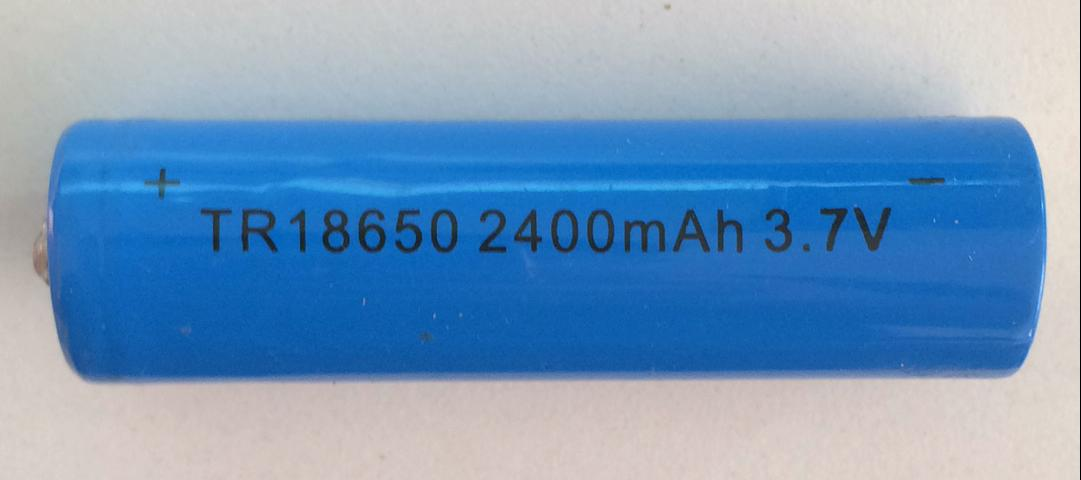
\includegraphics[width=0.5\textwidth]{./Figures/bateria.jpeg}			
	\caption{Batería TR18650 utilizada en el equipo}
	\label{fig:bateria}
\end{figure}

Teniendo en cuenta la eficiencia del 90\% y el porcentaje de descarga máxima de 51.35\%, la autonomía aprovechable de la batería será aproximadamente de 1109mAh, según lo calculado en la Ecuación \ref{eqn:autonomiaReal}.


\begin{equation} \label{eqn:autonomiaReal}
\begin{split}
autonomiaReal = autonomiaReal*eficiencia*porcentajeDescarga = \\ 2400mAh * 90\% * 51.35\% = 1109 mAh
\end{split}
\end{equation}

Este valor es cercano al consumo teórico calculado en \ref{eqn:consumoMedio}.
Se realizaron varias experiencias para verificar la autonomía del equipo y se obtuvieron en todas resultados similares. La duración de la batería fue de aproximadamente 22 horas. Puede verse la curva de descarga de una de las experiencias en la figura \ref{fig:descargaBateria}. En esta figura se decimaron las muestras obtenidas y se visualiza una medición cada media hora. El divisor resistivo de entrada del ADC conectado a la batería es de 330kOhm y 820kOhm, lo que da una relación de 0.287. Este valor se usó para convertir las muestras entregadas por el ADC a Volts.

\begin{figure} [!htpb]
    \centering
    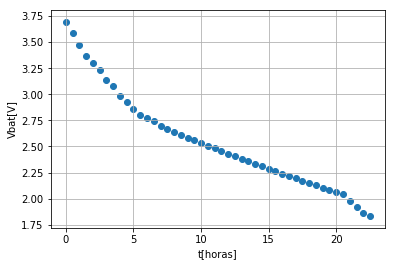
\includegraphics[width=\textwidth]{./Figures/descargaBateria.png}
    \caption{Descarga de la bateria durante experiencia}
    \label{fig:descargaBateria}
\end{figure}

Los requerimientos asociados a este caso de uso no son cubiertos completamente. Sin embargo, se puede solucionar colocando una batería de mayor autonomía como puede ser la indicada en \citep{rs2019}, que no fue adquirida por una cuestión de presupuesto.


\textbf{Caso de uso CU002: Configuración}

Para comprobar este caso de uso se inició con el equipo reiniciado por hardware. Se utilizó una tablet con Android y la aplicación Bluterm instalada. A través de la aplicación se enviaron los comandos para ingresar al modo configuración, y luego se modificaron cada uno de los parámetros, comprobando la escritura en las variables asociadas en RAM a través del debugger. Luego se realizaron diferentes mediciones para distintas configuraciones. Estas mediciones fueron realizadas con señales provistas por un generador de señales UTG4082A excitando la entrada del amplificador operacional. En la figura \ref{fig:confPGA} puede visualizarse la misma señal generada adquirida con dos ganancias de PGA diferentes (1 y 2). El setup para la experiencia puede visualizarse en la figura \ref{fig:confPGAexp}.

\begin{figure} [!htpb]
    \centering
    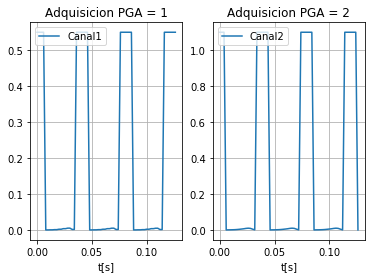
\includegraphics[width=\textwidth]{./Figures/confPGA.png}
    \caption{Señales adquiridas con PGA = 1 y PGA = 2}
    \label{fig:confPGA}
\end{figure}

\begin{figure} [!htpb]
    \centering
    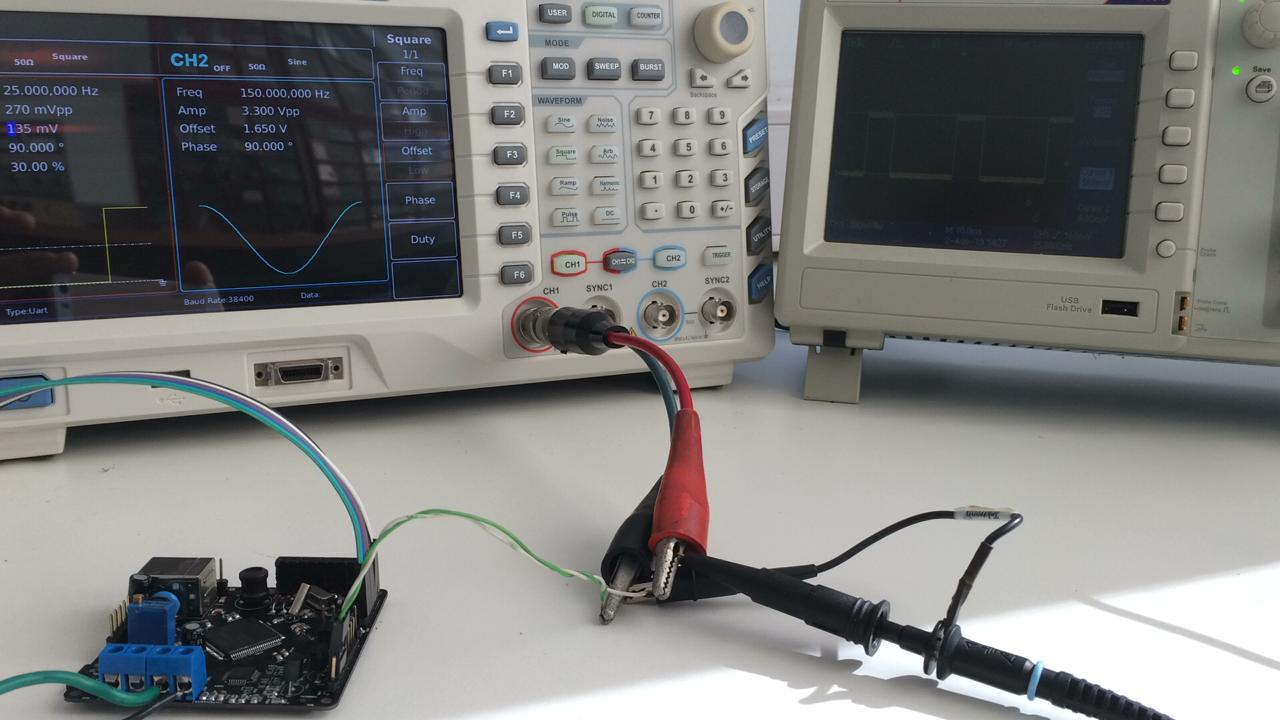
\includegraphics[width=\textwidth]{Figures/confPGAexp.jpeg}
    \caption{Señales adquiridas con PGA = 1 y PGA = 2}
    \label{fig:confPGAexp}
\end{figure}

Se realizó igualmente la configuración de habilitación de un solo canal (canal 1 y canal 2 por separado), la configuración de fecha y hora, y el muestreo a frecuencias de 500SPS, 250SPS y 125SPS.

También se realizó la rutina de calibración con uno de los sensores Königsberg, pero sin contar con un patrón de calibración de presión. Se comprobó unicamente la adquisición de valores diferentes de presión aplicando presión con el dedo y visualizando una medición mayor con su correspondiente incremento en el valor adquirido. El setup puede visualizarse en la figura \ref{fig:calibracion}. Resta comprobar la calibración con un patrón certificado de presión que sea adaptable a los sensores a utilizar. 

\begin{figure} [!htpb]
    \centering
    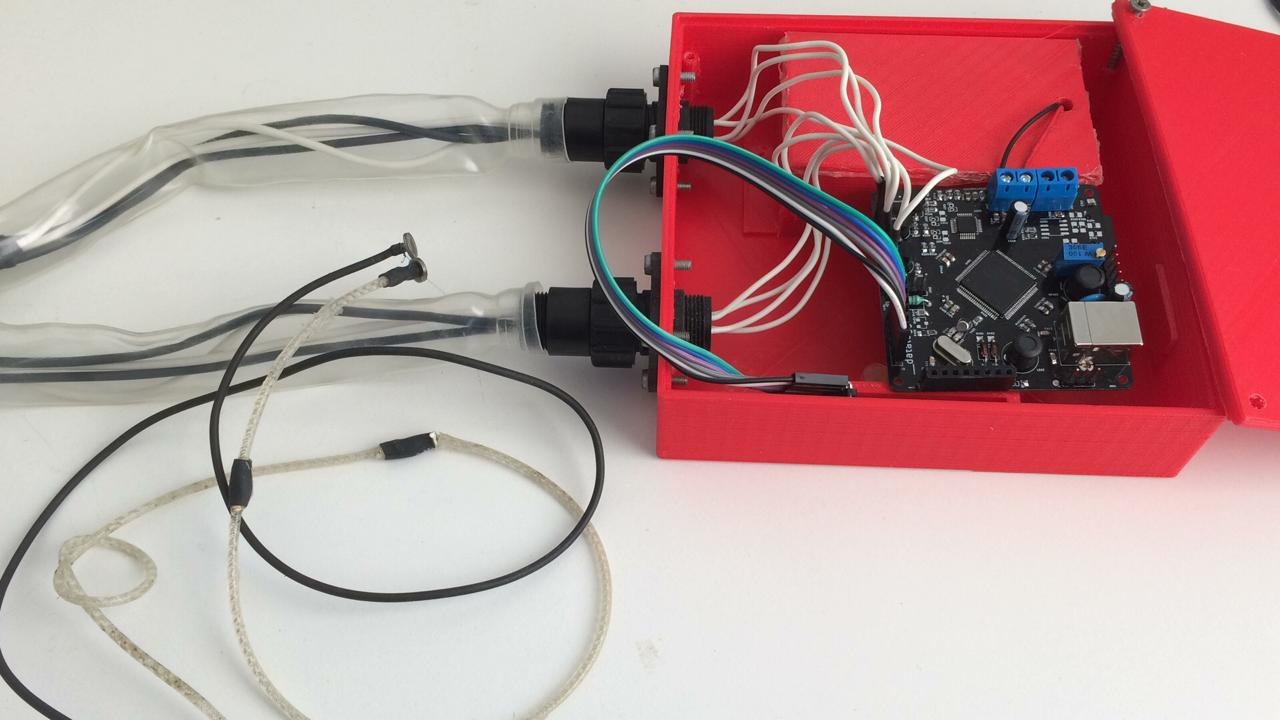
\includegraphics[width=\textwidth]{./Figures/calibracion.jpeg}
    \caption{Setup para calibración con sensores Königsberg}
    \label{fig:calibracion}
\end{figure}

\textbf{Caso de uso CU003: Experiencia}

Para este caso de uso se cargó la batería al 100\% y se operó el dispositivo desde una terminal con Android, utilizando la aplicación Bluterm. Por tratarse de una prueba de funcionamiento, se utilizó el mismo setup que en el caso de la calibración, es decir, con los sensores a presión atmosférica. Se ingresó en el modo de ''adquirir+enviar'', con la configuración por default, es decir, con los dos canales habilitados, el PGA en ganancia unitaria, y una frecuencia de muestreo de 500SPS. 

Se comprobó el correcto envío de muestras truncadas a 16 bits y decimadas a 100Hz para no sobrecargar el módulo Bluetooth. Luego se pasó al modo ''adquirir+enviar+almacenar'' y finalmente al modo ''adquirir+almacenar''. Después de esperar cinco minutos, se interrumpió la experiencia para comprobar el correcto almacenamiento en la memoria micro SD. 
Se volvió a comenzar la experiencia de la misma manera pero esta vez no se interrumpió el almacenamiento y se continuó por 20 horas, finalmente se dio por terminada la experiencia. 

Esta secuencia se repitió pero intercalando ingresos a través de la aplicación Bluterm para consultar el envío de la señal online, de manera de comprobar que la visualización de la señal no altere el almacenamiento en la SD.
Se repitió el mismo procedimiento por cuarta vez, pero ahora utilizando el generador de señales para comprobar la adquisición de una señal conocida. 

La estrategia elegida para almacenar las señales fue generar archivos de hasta 50Mb para evitar problemas de copia o corrupción. Para obtener mejor rendimiento de velocidad al escribir y menor volumen de datos, toda la información se guardó en formato binario. En cada uno de los archivos se guardo información que contiene un número de identificación de la experiencia autonumerado, un índice que comienza en cero y que indica el número de archivo generado abierto durante la experiencia, la fecha en que se guardó el archivo, hora de inicio del archivo, valor de ganancia del PGA, cantidad de canales habilitados, y valor de la frecuencia de muestreo. En cada una de las muestras se guardaron tres bytes por cada muestra por cada canal, ya que el ADC es de 24 bits y no tiene sentido guardar los cuatro bytes de la variable donde se almacenan los valores. Además para cada valor se guarda un byte correspondientes a la batería, truncando la muestra de 12 bits del ADC interno. La información de hora y fecha solamente se guarda en el encabezado, y no en cada muestra.

Para poder visualizar estos archivos se creó un script de python que reune esta información y la escribe en un formato legible, además compagina todos los archivos generados por la experiencia, graficando las señales. Este script se realizó con fines de desarrollo, ya que la aplicación para visualización e interfaz con el equipo no alcanza los objetivos del presente trabajo. 

Resta por realizar las pruebas de aceptación en un caso real, con un animal instrumentado. Esta experiencia no pudo ser realizada dado los costos e impedimentos operativos, pero se planifica realizar en el corto plazo.

\textbf{Caso de uso CU004: Descarga de datos y carga de batería}

En todos las experiencias realizadas para el CU003 se descargaron los archivos via USB. Para el tamaño de archivos que se maneja no hubo ningún inconveniente y el equipo respondió correctamente.

La carga de batería se realiza una corriente constante de 100mA, por lo que una carga completa con la batería totalmente descargada toma 24 horas. En todos los casos, luego de cargar la batería, se comprobó que la tensión final de carga sea 3.7V utilizando un tester UNI-T PRO UT195DS. 

\section{Ensayos adicionales}

También se realizaron ensayos para cubrir los requerimientos no funcionales, como los relacionados a las dimensiones físicas del equipo R2.1, R2.2 y R2.3. 

\begin{itemize}

\item R2.1: se hizo el pesaje del equipo en una balanza comercial. El peso con los sensores y el gabinete es de aproximadamente 366 gramos. 

\item R2.2: el gabinete del equipo mide 13.5cm x 12.8cm, más 1.5cm en la arista que contiene los conectores para los sensores. Este gabinete fue reutilizado de una versión anterior y cuenta con un gran espacio disponible en su interior, por lo que, si bien este requerimiento no fue cubierto en su totalidad, puede cumplirse realizando un nuevo gabinete, ya que el volumen que ocupa el circuito impreso y las baterías es mucho menor.

\item R2.3: durante todas las fases de los ensayos realizados se prestó especial atención a la temperatura de los compontentes. En ningún caso, ninguno de los componentes del circuito llegó tener una temperatura significativamente superior a la ambiental. Esto es consistente con el bajo consumo de corriente. El módulo Bluetooth es la única parte del sistema que llega a tener una temperatura apenas perceptiblemente mayor. 


\end{itemize}

\section{Resumen de los resultados} \label{resumenResultados}

A continuación en la Tabla \ref{tab:tablaConformidad} se sintetiza toda la información anterior: se muestra una lista de los requerimientos iniciales y su grado de conformidad.

\pagebreak

\footnotesize
\begin{longtable}[c]{lll}
\caption{Tabla de conformidad de requerimientos}\\ 
\hline
\textbf{REQ/CU} & \textbf{Conformidad} & \textbf{Observaciones}                                                                                                                                                                                                                                    \\ \hline
%
\endhead
%
R1.1            & Parcial              & \begin{tabular}[c]{@{}l@{}}Se debe colocar una batería \\ de mayor autonomía para superar\\ las 24hs de adquisición.\end{tabular}                                                                                                                         \\ \hline
R1.2            & Completa             & -                                                                                                                                                                                                                                                         \\ \hline
R2.1            & Completa             & -                                                                                                                                                                                                                                                         \\ \hline
R2.2            & Parcial              & \begin{tabular}[c]{@{}l@{}}Se debe cambiar el gabinete por\\ un nuevo diseño ya que el espacio\\ del circuito impreso y las baterías\\ es mucho menor al actual.\end{tabular}                                                                             \\ \hline
R2.3            & Completa             & -                                                                                                                                                                                                                                                         \\ \hline
R3.1            & Completa             & -                                                                                                                                                                                                                                                         \\ \hline
R3.2            & Completa             & -                                                                                                                                                                                                                                                         \\ \hline
R3.3            & Completa             & -                                                                                                                                                                                                                                                         \\ \hline
R4.1            & Parcial              & \begin{tabular}[c]{@{}l@{}}La resolución del ADS1292 y el nivel de\\ ruido del equipo permiten inferir que\\ este requisito es factible de cumplir, sin embargo,\\ es necesario realizar una calibración de los\\ sensores para comprobarlo.\end{tabular} \\ \hline
R4.2            & Completa             & \begin{tabular}[c]{@{}l@{}}Se realizaron pruebas con memorias de 2GB que \\ superan ampliamente el tamaño del paquete de \\ archivos generados por una experiencia de 24hs\\ con dos canales en 24 bits.\end{tabular}                                     \\ \hline
R4.3            & No Completa          & Este requerimiento resultó irrelevante en la práctica                                                                                                                                                                                                     \\ \hline
R5.1            & Completa             & -                                                                                                                                                                                                                                                         \\ \hline
R5.2            & Completa             & \begin{tabular}[c]{@{}l@{}}El ADS1292 cuenta con conversores A/D, que \\ toman las muestras con el mismo timer de entrada\end{tabular}                                                                                                                    \\ \hline
R6.1            & Completa             & -                                                                                                                                                                                                                                                         \\ \hline
R6.2            & Completa             & -                                                                                                                                                                                                                                                         \\ \hline
R6.3            & Completa             & -                                                                                                                                                                                                                                                         \\ \hline
R6.4            & Completa             & -                                                                                                                                                                                                                                                         \\ \hline
R6.5            & Completa             & -                                                                                                                                                                                                                                                         \\ \hline
R6.6            & Completa             & -                                                                                                                                                                                                                                                         \\ \hline
R6.7            & Completa             & -                                                                                                                                                                                                                                                         \\ \hline
R6.8             & Completa             & -                                                                                                                                                                                                                                                         \\ \hline
R6.9            & Completa             & -                                                                                                                                                                                                                                                         \\ \hline
R6.10           & Completa             & -                                                                                                                                                                                                                                                         \\ \hline
R6.11           & Completa             & -                                                                                                                                                                                                                                                         \\ \hline
R6.12           & Completa             & \begin{tabular}[c]{@{}l@{}}Se optó por registrar fecha y hora en el encabezado\\ de cada archivo en lugar de cada registro.\end{tabular}                                                                                                                  \\ \hline
R6.13           & Completa             & \begin{tabular}[c]{@{}l@{}}Se optó por generar varios archivos de 50Mb por cada \\ registro\end{tabular}                                                                                                                                                  \\ \hline
R6.14           & Completa             & -                                                                                                                                                                                                                                                         \\ \hline
R6.15           & Completa             & \begin{tabular}[c]{@{}l@{}}El led es SMD y se debería colocar en su lugar un \\ led THT visible desde fuera del gabinete.\end{tabular}                                                                                                                    \\ \hline
R7.1            & Completa             & -                                                                                                                                                                                                                                                         \\ \hline
R7.2            & Completa             & -                                                                                                                                                                                                                                                         \\ \hline
R7.3            & Completa             & -                                                                                                                                                                                                                                                         \\ \hline
R7.4            & Completa             & -                                                                                                                                                                                                                                                         \\ \hline
R7.5            & Completa             & -                                                                                                                                                                                                                                                         \\ \hline
R7.6            & Parcial              & \begin{tabular}[c]{@{}l@{}}Resta por realizar la calibración contra un patrón\\ de presión
\end{tabular}                                                                                                                                                     \\ \hline
\label{tab:tablaConformidad}
\end{longtable}
\normalsize

 
% Chapter Template

\chapter{Conclusiones} % Main chapter title

\label{Chapter5} % Change X to a consecutive number; for referencing this chapter elsewhere, use \ref{ChapterX}


%----------------------------------------------------------------------------------------

%----------------------------------------------------------------------------------------
%	SECTION 1
%----------------------------------------------------------------------------------------

\section{Conclusiones generales }

Para este proyecto se utilizaron en forma intensiva los contenidos y herramientas de la Carrera de Especialización en Sistemas Embebidos (CESE). Se pusieron en práctica técnicas de Gestión de Proyectos, documentación manual y automática del trabajo, sistema de versionado de software y hardware y conceptos fundamentales de Ingeniería de Software. Se emplearon conocimientos específicos sobre arquitectura del microcontrolador, modelos de programación, sistema operativo de tiempo real freeRTOS, protocolos de comunicación (BLE, SPI, USB, y de alto nivel) y testing unitarios, entre otros.

El trabajo se considera satisfactorio ya que se abarcaron gran parte de los objetivos, no solo funcionales, sino también académicos y de experiencia. Puntualmente se puede mencionar:

\begin{itemize}

\item Se logró un equipo funcional que cumple con gran parte de los requerimientos iniciales.

\item Se trabajó de una manera escalable, tomando criterios de calidad de software que permiten mantener y ampliar a futuro el firmware.

\item Se generó una apropiada documentación del trabajo, con la posibilidad de involucrar a estudiantes de la Universidad Favaloro para futuras mejoras como parte de su proyecto final.

\item El hardware se diseñó modularmente siguiendo conceptos aprendidos en el CESE, que permiten realizar nuevas versiones, correcciones y mejoras a futuro de una manera profesional.

\item Se utilizaron conceptos de gestión de proyectos que posiblitaron tener una visión más amplia y una experiencia muy rica, que da a lugar a extender las aplicaciones y alcances del dispositivo desarrollado a otras áreas de la ingeniería.

\item Es importante destacar que este proyecto tiene un adoptante concreto que utilizará el equipo para realizar investigaciones asociadas a la ingeniería biomédica. Es decir, es un proyecto de transferencia para equipar a un laboratorio de bioingeniería que planea utilizar el dispositivo para realizar mediciones en animales y desarrollar nuevos biomarcadores vasculares.

\end{itemize}

%----------------------------------------------------------------------------------------
%	SECTION 2
%----------------------------------------------------------------------------------------
\section{Próximos pasos}

Las instancias próximas a resolver son:

\begin{itemize}

\item Diseñar un gabinete a medida.

\item Probar el equipo en campo realizando varias experiencias.

\item Generar un software para interfaz Bluetooth y de PC.

\item Desarrollar el software de procesamiento y eventualmente generar índices de calidad que aseguren que las señales tengan una relación señal/ruido adecuada.

\end{itemize}


Además se planifican las siguientes mejoras a futuro relativas a:

\begin{itemize}

\item Agregar conectividad wifi para acceder al dispositivo remotamente.

\item Mejorar el consumo para poder realizar experiencias más prolongadas.

\item Reemplazar el conversor analógico digital ADS1292 por uno menos sofisticado que sea de menor precio.

\item Agregar entradas adicionales para medir otras variables de interés.

\end{itemize} 

%----------------------------------------------------------------------------------------
%	CONTENIDO DE LA MEMORIA  - APÉNDICES
%----------------------------------------------------------------------------------------

\appendix % indicativo para indicarle a LaTeX los siguientes "capítulos" son apéndices

% Incluir los apéndices de la memoria como archivos separadas desde la carpeta Appendices
% Descomentar las líneas a medida que se escriben los apéndices

%% Appendix A

\chapter{Appendix Title Here} % Main appendix title

\label{AppendixA} % For referencing this appendix elsewhere, use \ref{AppendixA}

Write your Appendix content here.
%\include{Appendices/AppendixB}
%\include{Appendices/AppendixC}

%----------------------------------------------------------------------------------------
%	BIBLIOGRAPHY
%----------------------------------------------------------------------------------------

\Urlmuskip=0mu plus 1mu\relax
\raggedright
\printbibliography[heading=bibintoc]

%----------------------------------------------------------------------------------------

\end{document}  
